\documentclass[border=4pt]{standalone}

% --- packages (mirror these in attention.meta.json "requires") ---
\usepackage{tikz}
\usetikzlibrary{positioning, arrows.meta}

% --- palette (canonical source: reference/color-palettes/color-palettes.md; light variant) ---
\definecolor{otblue}{HTML}{0072B2}
\definecolor{otorange}{HTML}{E69F00}
\definecolor{otteal}{HTML}{009E73}
\definecolor{otpurple}{HTML}{CC79A7}
\definecolor{otgray}{HTML}{5A5A5A}

\begin{document}
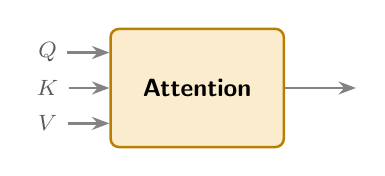
\begin{tikzpicture}[line width=0.9pt, >={Stealth[length=2.2mm]}]
  % attention block
  \node[rounded corners=3pt, draw=otorange!80!black, fill=otorange!20,
        minimum width=2.2cm, minimum height=1.5cm,
        font=\sffamily\small\bfseries] (attn) {Attention};
  % Q, K, V inputs
  \foreach \lab/\y in {Q/0.45, K/0, V/-0.45}{
    \node[font=\sffamily\footnotesize, text=otgray] (\lab) at (-1.9,\y) {$\lab$};
    \draw[->, draw=otgray!75] (\lab.east) -- (attn.west |- \lab);
  }
  % output
  \draw[->, draw=otgray!75] (attn.east) -- ++(0.9,0);
\end{tikzpicture}
\end{document}
